\newpage % Эта команда начинает новую страницу
\chapter{Тема лекции}% Эта команда начинает первую лекцию. В фигурных скобках нужно
% записать тему лекции. Эта тема лекции автоматически получит порядковый номер и
% автоматически добавится в раздел <<Содержание>>. Лекций можно создавать сколько угодно.
% Для создания новой лекции скопируйте и вставьте (или наберите с клавиатуры) команду
% \chapter{Тема лекции} в любую часть рабочего файла. Можете смело менять местами лекции --
% вся нумерация после очередной компиляции поменяется автоматически.

% При необходимости здесь можно разместить любой текст

\section{Название параграфа}% Эта команда начнет раздел, который будем далее условно называть
% параграф. В роли параграфа будет выступать структурная часть лекции (отдельный раздел,
% вопрос и т.п.). В фигурных скобках нужно вписать название параграфа. Параграф автоматически
% получит порядковый номер, который будет состоять из двух чисел, разделенных точкой.
% Первое число -- порядковый номер лекции, второе число -- порядковый номер параграфа в
% пределах лекции. Параграфов можно создавать сколько угодно. Для создания нового параграфа
% скопируйте и вставьте (или наберите с клавиатуры) команду \section{Название параграфа} в
% любую часть рабочего файла. Можете смело менять местами параграфы, переносить их из одной
% лекции  в другую -- вся нумерация после очередной компиляции поменяется автоматически.

% При необходимости здесь можно разместить любой текст

\subsection{Название подпараграфа}% Эта команда начинает подраздел, который далее будем
% условно называть подпараграфом. В фигурных скобках нужно вписать название подпараграфа.
% Подпараграф автоматически получит порядковый номер, который будет состоять из трех
% чисел, разделенных точками. Первое число -- порядковый номер лекции, второе число --
% порядковый номер параграфа, третье число -- порядковый номер подпараграфа. Подпараграфов
% можно создавать сколько угодно. Для создания нового подпараграфа скопируйте и вставьте
% (или наберите с клавиатуры) команду \subsection{Название подпараграфа} в любую часть
% Рабочего файла. Можете смело менять подпараграфы местами, переносить их из одного
% параграфа в другой (даже другой параграф другой лекции) -- вся нумерация после очередной
% компиляции поменяется автоматически.

Теперь можно приступать к формированию первой лекции Вашего учебно-методического
комплекса. Внимательно прочитайте все рекомендации <<Руководства пользователю>>.

Несколько важных моментов из <<Руководства пользователю>> мы продублируем и здесь.

Начнем с самого главного -- примера оформления программного кода в \LaTeX:

\begin{lstlisting}
    //example of simple C++ program
    void main()
    {
        int i = 12;
        int a = i + 100;
        cout << "Hello, world!";
    }
\end{lstlisting}

Определенные части текста (не содержащие формул, таблиц и иллюстраций -- о них речь пойдет
ниже) могут быть скопированы и вставлены  в рабочий документ из любого
другого текстового редактора. Исходный текст документа не должен содержать переносов
(\LaTeX~ создат их сам). Слова должны отделяться
друг от друга пробелами, но при этом \LaTeX у все-равно, сколько именно пробелов Вы
оставили между
словами, все пробелы \LaTeX~воспримет как один пробел
 (чтобы вручную управлять пробелами между словами можно использовать символ
$\sim$, который называют неразрывным пробелом).
 Конец строки также воспринимается как пробел.
Отдельные абзацы должны быть отделены друг от друга пустыми строками (опять-таки все равно,
сколько именно пустых строк стоит между абзацами, важно, чтобы была хоть одна).

Приведем пример создания определения:

\begin{opr}\label{oprperv} \rm Первообразной функции $f$ на множестве $X{\subset}D(f)$
называется такая функция $F,$ определённая на $X,$ что для любой
точки $x\in{X}$ будет выполняться равенство
  $$F'(x)=f(x).$$
\end{opr}

Пример создания теоремы:
\begin{theorem}\label{theorperv} Если функция $F$ является первообразной для функции $f$
на промежутке $X,$ то:

   {\rm a)} $F(x)+C$ также является первообразной для функции $f$ на промежутке
$X,$ где $C$ --- произвольная действительная постоянная;

    {\rm б)} для любой
другой первообразной $\Phi(x)$ функции $f$ на промежутке $X$
существует такая действительная константа $C,$ что
  $$\Phi(x)=F(x)+C.$$
\end{theorem}

Приведем пример создания гиперссылок на определение \ref{oprperv}  и теорему \ref{theorperv}.

Чтобы научиться легко создавать любые гиперссылки, внимательно прочитайте <<Руководство
пользователю>>.

Теперь приведем пример создания метки {\color{green}\hypertarget{metkatext}{на часть текста}}.

Теперь создадим гиперссылку на словосочетание <<часть текста>>. Пусть эта гиперссылка
состоит из слов <<\hyperlink{metkatext}{текстовая гиперссылка}>>

Пример создания списка:
\begin{enumerate}
\item текст;
\item текст;
\item текст.
\end{enumerate}

Пример создания следствия:
\begin{corollary}{\rm(Свойство линейности)}. Если на промежутке $I$ существуют $\int
f_k(x)dx, k=\overline{1,n}$, а $\alpha_k$ --- произвольные
действительные константы, причем хотя бы одна из них отлична от
нуля, то на $I$ существует $$\int\left(\sum_{k=1}^n \alpha_k
f_k(x)\right)dx=\sum_{k=1}^n \alpha_k
\int{f_k(x)dx}.$$\end{corollary}

Пример вставки рисунка 1n.png из папки <<pic>>/<<images>>.
\begin{figure}[h!]\center
  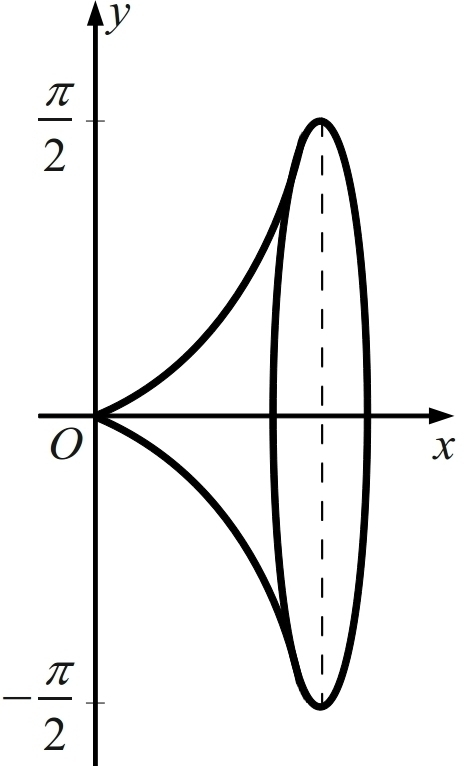
\includegraphics[height=5.11cm,bb=0 0 464 766]{1n.jpg}
   \caption{Тело вращения}\label{ris1}
\end{figure}

Пример вставки гиперссылки на запуск звукового файла 2.wma из папки <<media>>:
Послушаем \href{run:media/2.wma}{музыку}?

Пример вставки гиперссылки на запуск видео файла film.wmv из папки <<media>>:
\href{run:media/film.avi}{видеофильм}?

\section{Справочная информация}

Этот параграф можно назвать как угодно. Мы установим на первую страницу этого параграфа
метку \label{mybutton}, которая является <<мишенью>> Вашей кнопки на интерактивной панели
(описание процесса ее создания смотрите выше в комментариях).
\begin{enumerate}% Эта команда начинает список
\item Важная информация.
\item Очень важная информация.
\end{enumerate}% Эта команда завершает список

Если теперь скомпилировать <<Рабочий файл>>, то запустив электронный
учебник (файл UMK.pdf) и нажав на кнопку <<Ваша кнопка>> на интерактивной
панели, Вы попадете на эту страницу.

%--------------------------------------------------------------------------------------------

\section*{Вопросы и задания для самоконтроля}% Этот раздел будет состоять из вопросов
% и заданий для самоконтроля.
\addcontentsline{toc}{struct}{Вопросы и задания для самоконтроля}% Эта команда
% добавляет название раздела в раздел <<Содержание>>

Здесь можете привести список вопросов и заданий для самоконтроля:
\begin{enumerate}% Эта команда начинает список
\item Вопрос или задание.
\item Вопрос или задание.
\item Вопрос или задание.
\item Вопрос или задание.
\end{enumerate}% Эта команда завершает список

А можете подготовить с помощью программы IrenEditor (см. <<Руководство пользователю>>)
тестовое задание для самоконтроля, сохранить его в папку
<<test>>, назвав, например, lk1.exe, и создать на него метку с помощью
команды (см. <<Руководство пользователю>>): \href{run:test/lk1.exe}{Пройдем тестирование?}
